\chapter{\Peano's architecture}
\label{chapter:architecture}


\begin{center}
  \includegraphics[width=0.6\textwidth]{../src/peano4/architecture-layers.pdf}
\end{center}


\noindent
\Peano\ is organised into layers, and only the bottom two layers are found in
all \Peano\ applications.
I discuss the layers bottom-up:

\begin{itemize}
  \item[tarch] The technical architecture is a set of loosly coupled building
  blocks that hide away technical details. There's for example a namespace to
  handle multicore parallelism, a logging component, or a collection of
  primitive linear algebra routines for small problems. It is written solely in
  C++ and its purpose is to hide away third-party dependencies such as OpenMP
  or MPI. I originally designed it as a stand-alone thing which is not tied to
  Peano though I'm not aware of any other project that currently uses it. The
  layer is pronounced ``T Arch'' and is encapsulated in a namespace
  \texttt{tarch}, as I didn't want to write the full name ``technical
  architecture'' every time.
  \item[peano4] The namespace \texttt{peano4} hosts the \Peano\ core. It is
  entirely written in C++ (using the tarch) and holds the heart and brain of the
  code, i.e.~all the data management, the tree traversals and the domain
  decomposition.
  \item[Native] \Peano\ applications use solely the core and the tarch. I write
  such codes from time to time myself, but it is a tedious task as all the user
  data management and management of ``which routine is used when'' has to be
  programmed manually.
  \item[Other projects] can obviously supplement the core and tarch with further
  routines using either of the two components. The most prominent project
  extending the core is maybe \ExaHyPE. The illustration here is not 100\%
  correct as noone forces developers to write these extensions in C++. In
  practice however, most of them are (with small Fortran imports, e.g.). 
  \item[Native projects] can use the core extensions using C++. Most projects
  (like ExaHyPE) however do all offer a more abstract interface (see below).
  \item[Python API] \Peano\ offers a Python API which is basically a code
  generator yielding lots of C++ snippets that plug into the core and use the
  tarch. Some of my examples use this Python API only.
  \item[API extensions] are also offered by other projects such as ExaHyPE or
  ExaClaw. They often supplement the core Python API with further classes.
\end{itemize}


\section*{Organisation of guidebook}

The guidebook is split into parts anticipating the layered architecture of the
code.

One part discusses the C++ features offered both by the
tarch and \Peano's core.
This part is very useful for anybody who writes C++ code within \Peano, and it
also gives information how \Peano\ works under the hood. 
Some developers might be able to work completely without the details described
in this part.
However, as soon as you have some linear algebra operations for example, you
might want to be familiar with the core features.


One part gives some examples how to work with the Python API. 
Most people who use this API won't be able to stick to Python only, but:
The API is powerful mechanism generating C++ glue code and C++
stubs.
The latter still have to be befilled with actual computations by the user.
So the API takes away the responsibility to assemble the application, but it
does not completely hide away C++.


One part discusses how to use big projects built on top of
\Peano\ that have a very high abstraction level.
\ExaHyPE/ExaClaw are the two biggest fishes at the moment.
If you work on this level, you can likely completely ignore the other Python
details and a lot of the C++ low level details for quite a while.


Another part finally discusses how to extend the Python API.
This is relevant for all the developers that do not only want to create a code
with \Peano\ but want to make their stuff easily available to others.
After that, I spend a few pages to summarise design decisions (rationale)
underrlying the code.
This might help to understand why certain things work the way they do.


An appendix gives further information on particular machines, file formats, and
so forth. 
It hosts an FAQ and tips how to combine/use \Peano\ with other tools.
